\documentclass[11pt,preprint, authoryear]{elsarticle}

\usepackage{lmodern}
%%%% My spacing
\usepackage{setspace}
\setstretch{1.2}
\DeclareMathSizes{12}{14}{10}{10}

% Wrap around which gives all figures included the [H] command, or places it "here". This can be tedious to code in Rmarkdown.
\usepackage{float}
\let\origfigure\figure
\let\endorigfigure\endfigure
\renewenvironment{figure}[1][2] {
    \expandafter\origfigure\expandafter[H]
} {
    \endorigfigure
}

\let\origtable\table
\let\endorigtable\endtable
\renewenvironment{table}[1][2] {
    \expandafter\origtable\expandafter[H]
} {
    \endorigtable
}


\usepackage{ifxetex,ifluatex}
\usepackage{fixltx2e} % provides \textsubscript
\ifnum 0\ifxetex 1\fi\ifluatex 1\fi=0 % if pdftex
  \usepackage[T1]{fontenc}
  \usepackage[utf8]{inputenc}
\else % if luatex or xelatex
  \ifxetex
    \usepackage{mathspec}
    \usepackage{xltxtra,xunicode}
  \else
    \usepackage{fontspec}
  \fi
  \defaultfontfeatures{Mapping=tex-text,Scale=MatchLowercase}
  \newcommand{\euro}{€}
\fi

\usepackage{amssymb, amsmath, amsthm, amsfonts}

\def\bibsection{\section*{References}} %%% Make "References" appear before bibliography


\usepackage[round]{natbib}

\usepackage{longtable}
\usepackage[margin=2.3cm,bottom=2cm,top=2.5cm, includefoot]{geometry}
\usepackage{fancyhdr}
\usepackage[bottom, hang, flushmargin]{footmisc}
\usepackage{graphicx}
\numberwithin{equation}{section}
\numberwithin{figure}{section}
\numberwithin{table}{section}
\setlength{\parindent}{0cm}
\setlength{\parskip}{1.3ex plus 0.5ex minus 0.3ex}
\usepackage{textcomp}
\renewcommand{\headrulewidth}{0.2pt}
\renewcommand{\footrulewidth}{0.3pt}

\usepackage{array}
\newcolumntype{x}[1]{>{\centering\arraybackslash\hspace{0pt}}p{#1}}

%%%%  Remove the "preprint submitted to" part. Don't worry about this either, it just looks better without it:
\makeatletter
\def\ps@pprintTitle{%
  \let\@oddhead\@empty
  \let\@evenhead\@empty
  \let\@oddfoot\@empty
  \let\@evenfoot\@oddfoot
}
\makeatother

 \def\tightlist{} % This allows for subbullets!

\usepackage{hyperref}
\hypersetup{breaklinks=true,
            bookmarks=true,
            colorlinks=true,
            citecolor=blue,
            urlcolor=blue,
            linkcolor=blue,
            pdfborder={0 0 0}}


% The following packages allow huxtable to work:
\usepackage{siunitx}
\usepackage{multirow}
\usepackage{hhline}
\usepackage{calc}
\usepackage{tabularx}
\usepackage{booktabs}
\usepackage{caption}


\newenvironment{columns}[1][]{}{}

\newenvironment{column}[1]{\begin{minipage}{#1}\ignorespaces}{%
\end{minipage}
\ifhmode\unskip\fi
\aftergroup\useignorespacesandallpars}

\def\useignorespacesandallpars#1\ignorespaces\fi{%
#1\fi\ignorespacesandallpars}

\makeatletter
\def\ignorespacesandallpars{%
  \@ifnextchar\par
    {\expandafter\ignorespacesandallpars\@gobble}%
    {}%
}
\makeatother

\newlength{\cslhangindent}
\setlength{\cslhangindent}{1.5em}
\newenvironment{CSLReferences}%
  {\setlength{\parindent}{0pt}%
  \everypar{\setlength{\hangindent}{\cslhangindent}}\ignorespaces}%
  {\par}


\urlstyle{same}  % don't use monospace font for urls
\setlength{\parindent}{0pt}
\setlength{\parskip}{6pt plus 2pt minus 1pt}
\setlength{\emergencystretch}{3em}  % prevent overfull lines
\setcounter{secnumdepth}{5}

%%% Use protect on footnotes to avoid problems with footnotes in titles
\let\rmarkdownfootnote\footnote%
\def\footnote{\protect\rmarkdownfootnote}
\IfFileExists{upquote.sty}{\usepackage{upquote}}{}

%%% Include extra packages specified by user

%%% Hard setting column skips for reports - this ensures greater consistency and control over the length settings in the document.
%% page layout
%% paragraphs
\setlength{\baselineskip}{12pt plus 0pt minus 0pt}
\setlength{\parskip}{12pt plus 0pt minus 0pt}
\setlength{\parindent}{0pt plus 0pt minus 0pt}
%% floats
\setlength{\floatsep}{12pt plus 0 pt minus 0pt}
\setlength{\textfloatsep}{20pt plus 0pt minus 0pt}
\setlength{\intextsep}{14pt plus 0pt minus 0pt}
\setlength{\dbltextfloatsep}{20pt plus 0pt minus 0pt}
\setlength{\dblfloatsep}{14pt plus 0pt minus 0pt}
%% maths
\setlength{\abovedisplayskip}{12pt plus 0pt minus 0pt}
\setlength{\belowdisplayskip}{12pt plus 0pt minus 0pt}
%% lists
\setlength{\topsep}{10pt plus 0pt minus 0pt}
\setlength{\partopsep}{3pt plus 0pt minus 0pt}
\setlength{\itemsep}{5pt plus 0pt minus 0pt}
\setlength{\labelsep}{8mm plus 0mm minus 0mm}
\setlength{\parsep}{\the\parskip}
\setlength{\listparindent}{\the\parindent}
%% verbatim
\setlength{\fboxsep}{5pt plus 0pt minus 0pt}



\begin{document}



\begin{frontmatter}  %

\title{The Analysis of Core PCA drivers for Currency Rates}

% Set to FALSE if wanting to remove title (for submission)




\author[Add1]{Jessica Van der Berg}
\ead{20190565@sun.ac.za}





\address[Add1]{Stellenbosch Univeristy, South Africa}

\cortext[cor]{Corresponding author: Jessica Van der Berg}

\begin{abstract}
\small{
Using principal component analysis, I identify the core driving factors
of emerging and developing market currency rates. I analyse 33
currencies from 1994-03-30 to 2021-10-29. I find that the first
principal component is related to commodities, especially oil. The
second principal component relates to political instability and the
absence of violence/terrorism. The third principal component relates to
some Asian factor. These factors can be used in further studies to make
predictions about currency rates and determine whether they are
under/overvalued.
}
\end{abstract}

\vspace{1cm}


\begin{keyword}
\footnotesize{
PCA \sep Emerging Market \sep Developing Market \\
\vspace{0.3cm}
}
\footnotesize{
\textit{JEL classification} L250 \sep L100
}
\end{keyword}



\vspace{0.5cm}

\end{frontmatter}



%________________________
% Header and Footers
%%%%%%%%%%%%%%%%%%%%%%%%%%%%%%%%%
\pagestyle{fancy}
\chead{}
\rhead{Financial Econometric Project}
\lfoot{}
\rfoot{\footnotesize Page \thepage}
\lhead{}
%\rfoot{\footnotesize Page \thepage } % "e.g. Page 2"
\cfoot{}

%\setlength\headheight{30pt}
%%%%%%%%%%%%%%%%%%%%%%%%%%%%%%%%%
%________________________

\headsep 35pt % So that header does not go over title




\hypertarget{introduction}{%
\section{\texorpdfstring{Introduction
\label{Introduction}}{Introduction }}\label{introduction}}

The foreign exchange market is the largest financial market in the
world, and it is extremely liquid. It provides investors with a lot of
flexibility, since there are no restrictions on the total amount of
money that one individual can use for investing. Furthermore, there is
also no regulation of the market, implying that it operates on a 24-7
basis \protect\hyperlink{ref-tana}{Tanamarttayarat}
(\protect\hyperlink{ref-tana}{2018}). However, investing in currency
rates have often been overlooked as a potential resource of returns for
a variety of reasons. One reason is that currency rates can be
challenging to model. The underlying source of value of a currency rate
is elusive \protect\hyperlink{ref-pojar}{Pojarliev \& Levich}
(\protect\hyperlink{ref-pojar}{2013}). An economic model for currency
valuation often uses fundamental macroeconomic variables, such as real
income or national money supply, to estimate the fair value of the
currency rate. However, these models are often overly restrictive and
account for country-specific macroeconomic variables, making it nearly
impossible to replicate the results across currency rates. Therefore, an
economic model that works well for a specific currency or period may not
necessarily work well for other currencies or periods. There is also the
risk of central bank intervention in currency rates which deters
investors from investing. However, profit opportunities in the currency
market are available but are subject to a high level of risk and are
mostly suitable for specialist \protect\hyperlink{ref-pono}{Ponomareva,
Sheen \& Wang} (\protect\hyperlink{ref-pono}{2019}).

Taking these shortcomings and strengths into account, this paper uses
principal component analysis to analyse the relationship between
currency rates and macroeconomic variables. By examining 33 emerging and
developing market currency rates, the paper concludes that shocks to
commodity prices, such as an oil price shock, political instability and
the Asian economy are all important macroeconomic variables that account
for most of the variation in currency rates.

The paper is structured as follows: Section 2 briefly discusses the
data, methodology and some descriptive statistics of the principal
component analysis. Section 3 provides an in-depth discussion about the
core principal component drivers for currency rates. Section 4 forecasts
the three most traded currency rates. Finally, section 5 concludes.

\hypertarget{pca-analysis}{%
\section{PCA Analysis}\label{pca-analysis}}

This paper analysis daily currency rates from the 30th of March 1990
till the 29th of October 2021. The currency rates are all relative to
USD. The currency rates were split into emerging and developing markets
according to the Morgan Stanley Capital International (MSCI) 2021 annual
market classification. Frontier and standalone markets were not
considered. Table \ref{cncy} in appendix A displays the countries under
consideration. Ultimately, 12 developing markets and 21 Emerging markets
were analysed. Figure \ref{data} in appendix A plots the rates of all 33
currencies.

Analysing 41 emerging and developing market currency rates result in
very large datasets that need interpretation. Empirical techniques have
been developed to decrease the dimensionality of a large dataset. One
such empirical technique is principal component analysis (PCA), which is
used to reduce the dimensionality of large datasets in an interpretable
way while minimizing information loss. To achieve this, a new
uncorrelated variable is created, known as the principal component,
which maximizes the variance \protect\hyperlink{ref-jolli}{Jolliffe \&
Cadima} (\protect\hyperlink{ref-jolli}{2016}). The PCA yields 33
orthogonal principal components. To examine the relative importance of
each principal component, I compare the scale of the eigenvalues of the
variance-covariance matrix. The results are displayed in the scree plot
in figure \ref{scree}.

\begin{figure}[h]
\centering
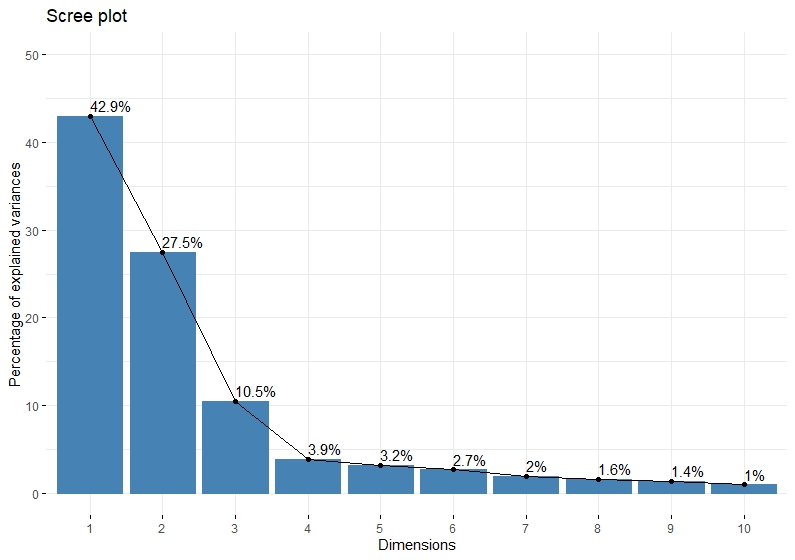
\includegraphics[scale=0.7]{scree.jpg}
\caption{Scree plot}
\label{scree}
\end{figure}

The scree plot indicates that the first principal component explains
42.9 percent of the variability, the second explains 27.5 percent and
the third explains 10.5 percent. Therefore, the first three principal
components explain 80.9 percent of the total variation. Figure
\ref{pcpc} displays the first principal component. There is a drastic
increase around 2008 during the financial crisis. This reflects the
sharp appreciation of the USD against most currencies. The US dollar
strengthens due to the global \emph{flight to safety} into US Treasury
bills as well as the reversal of carry trades
\protect\hyperlink{ref-mcc2009}{McCauley \& McGuire}
(\protect\hyperlink{ref-mcc2009}{2009}). The same pattern can be seen
during 2020 when the COVID\_19 crisis was in full effect, however, the
extent is much smaller.

\begin{figure}
\centering
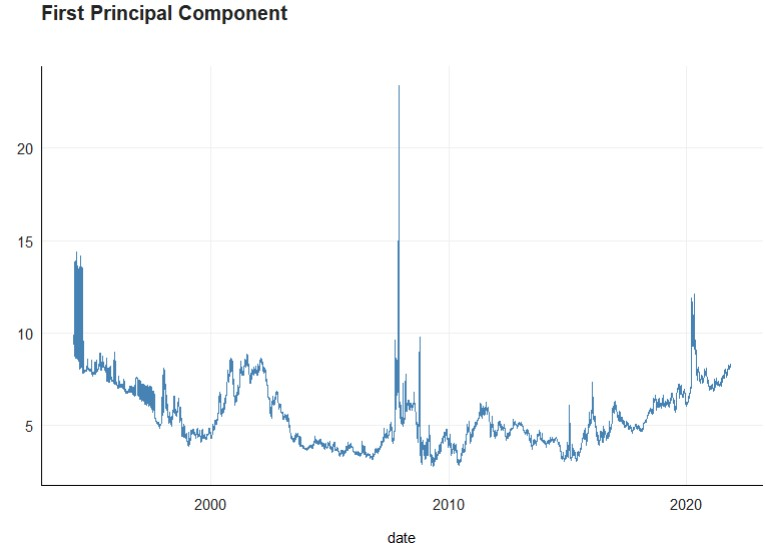
\includegraphics[scale=0.9]{pc1.jpg}
\caption{First Principal Component }
\label{pcpc}
\end{figure}

\hypertarget{identifying-common-drivers}{%
\section{Identifying Common Drivers}\label{identifying-common-drivers}}

The principal component is used to analyse the driving forces. By
comparing the eigenvalues of the variance-covariance matrix in the
previous section, I determined that the first three principal components
explain the majority of the total variance of the currency rates. In
this section, I examine the correlation between the first three
principal component and the currency rates, as well as provide economic
interpretations around the core driving factors that affect currency
rates.

Table \ref{pca1} in appendix B shows the correlation and p-value for the
first principal component (PC1). The country that has the highest
positive correlation with PC1 is Hungary (HUF), which is a net importer
of crude petroleum. Saudi Arabia (SAR) and the United Arab Emirates
(AED) are two of the top exporting countries. China (CNY) is the only
country with a negative correlation with PC1, with its top import being
refined petroleum. Therefore, one would expect that the oil price is one
of the core PCA drivers for currencies.

Oil is an extremely important, non-renewable resource. The demand and
price for oil tend to drastically increase with world economic
development \protect\hyperlink{ref-li2015}{Li \& Ma}
(\protect\hyperlink{ref-li2015}{2015}). Crude oil is quoted in the U.S
dollar, therefore there is a direct relationship between the two.
Theoretically, an appreciation in the US dollar should cause a decrease
in the price of oil. However, empirical research has found contradicting
results, indicating a bi-directional causality relationship between oil
and currency rates \protect\hyperlink{ref-beck2020}{Beckmann, Czudaj \&
Arora} (\protect\hyperlink{ref-beck2020}{2020}). Fluctuations in the oil
prices are diverse and unique, depending on whether a country is a net
importing or net exporting country. For oil-importing countries,
\protect\hyperlink{ref-castro}{Castro \& Jimenez-Rodriguez}
(\protect\hyperlink{ref-castro}{2020}) found that an oil price shock
leads to depreciation of the home currency in the short run, however,
the long-run effects are diverse.

For oil-exporting countries, it has been empirically proven that
instability in the oil price does not have a significant effect on
economic growth. Table \ref{pca1} supports the results of
\protect\hyperlink{ref-can2021}{Candila, Maximov, Mikhaylov, Moiseev,
Senjyu \& Tryndina} (\protect\hyperlink{ref-can2021}{2021}) who found a
much stronger correlation for oil-importing countries. China is a unique
case has it is one of the largest importers and exporters of oil.
\protect\hyperlink{ref-li2015}{Li \& Ma}
(\protect\hyperlink{ref-li2015}{2015}) found a non-linear causality
between the oil price and the RMB exchange rate. This indicates that
movement in the price of oil can cause co-movement of RMB with a
one-month lag. Since the relationship between the oil price and currency
rates are diverse and unique, policymakers should react with caution
when examining currency rate pressure.

Table \ref{pca2} in appendix B displays the correlation and the p-value
for the second principal component (PC2). The countries that have the
highest correlation with PC2 are, amongst others, Singapore (SGD), New
Zealand (NZD), Australia (AUD) and Canada (CAD), all developing market
economies. The countries with the lowest correlation with PC2 are Turkey
(TRY), Egypt (EGP) and Mexico (MXN). This suggest that the PC2 is
related to political stability. Countries with a high political
stability and absence of violence/terrorism ranking are highly
correlated with PC2, whereas countries with a low ranking are often
negatively correlated with PC2.

A country with a high political stability ranking offer much more safe
and attractive investment opportunity for foreign investors. This
implies that political stability has a significant effect on currency
rates. Political unrest, such a serious allegation into government
conduct can contribute to the destabilization of an economy, which will
weaken currency rates. Changes in currency rates are known as
\emph{exchange rate risk} which accounts for uncertainty in movement in
the exchange rate between the home and receiver country
\protect\hyperlink{ref-higg}{Higgins, Hysenbegasi \& Pozo}
(\protect\hyperlink{ref-higg}{2004}).

Although the effect of political instability is profound,
\protect\hyperlink{ref-levis}{Levis}
(\protect\hyperlink{ref-levis}{1979}) found that the relationship
between political instability in developed countries and foreign direct
invest are highly significant in the short run, but not the long run.
This would suggest that foreign investors adjust quickly to new
developments and that political stability should be considered in
conjunction with numerous other relevant factors.

The correlation and the p-value for the third principal component is
represented in Table \ref{pca3} in appendix B. The countries with the
largest correlation all appear in Asia and the countries with the lowest
correlation are all developed market. This implies that the third
principal component is an Asia-specific factor. Over the past few areas,
Asian countries have experienced phenomenal growth, which has created
profitable opportunities for foreign investors.

\hypertarget{forecasting}{%
\section{Forecasting}\label{forecasting}}

Forecasting currency rates is important to many fields such as
international business and monetary policy. However, it is challenging
to obtain accurate forecasts due to the fluctuations caused by political
instability, shocks to commodity prices and economic events. From an
investing point of view, an accurate forecast reduces risk related to
international investments as well as maximizes returns. Monetary policy
also depends on an accurate forecast of currency rates, as changes in
the interest rate can either appreciate or depreciate the home currency.
Changes in currency rate affect trade, which affects economic growth.
Therefore, an accurate currency forecast can assist authorities to
implement effective policies that boost economic growth
\protect\hyperlink{ref-shen}{Shen, Lee, Liu, Chang \& Yang}
(\protect\hyperlink{ref-shen}{2021}). In this section, I attempt to
forecast the three most traded currencies: the Euro (EU), the Pound
sterling (GBP) and the Japanese yen (JPY). Figure \ref{for} displays the
currency rate for the three currencies, all relative to USD.

\begin{figure}
\centering 
\begin{minipage}[t]{8.2cm} 
\centering 
 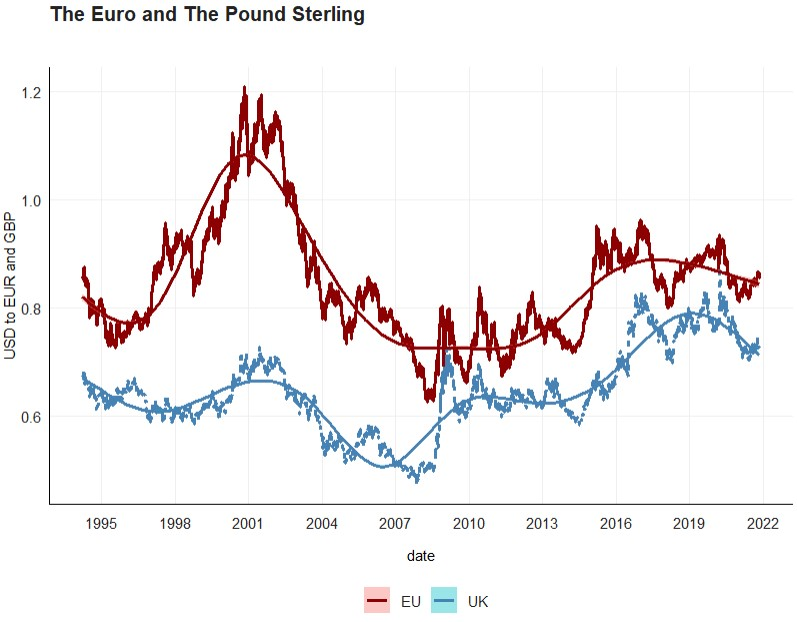
\includegraphics[width=\linewidth]{for1.jpg} 
 \end{minipage} 
 \hspace{0.1cm} 
 \begin{minipage}[t]{8.2cm} 
 \centering 
 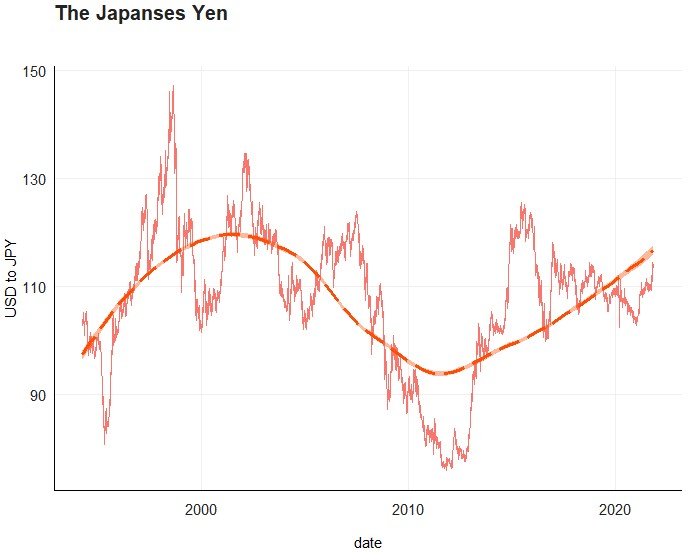
\includegraphics[width=\linewidth]{for2.jpg} 
 \end{minipage}
\caption{The three most traded currencies}
\label{for}
\end{figure}

I employ a 30 period ahead Autoregressive Integrated Moving Average
(ARIMA) model to forecast currency rates.
\protect\hyperlink{ref-akin}{Akincilar, TEMIZ \& Sahin}
(\protect\hyperlink{ref-akin}{2011}) found that the ARIMA model performs
relatively well when compared to other forecasting methods. Figure
\ref{for1} and figure \ref{for2} show the forecasting results for the
selected currencies with a 95 per cent upper and lower bound. The
forecast results indicate that the USD/GBP rate is forecasted to
decrease, implying that the Pound sterling is going to strengthen.
However, the actual data shows the opposite effect, the GBP currency
rate weakened.

The forecast results indicate that the USD/EU rate is forecasted to
increase slightly, implying that the euro is going to decrease. Actual
data support this forecast. The forecast results indicate that the
USD/JPY rate is forecasted to decrease slightly, implying that the Pound
sterling is going to strengthen. Actual data shows that the currency
rate remained relatively stable, making the forecast results mostly
accurate. The results should be further investigated to conclude on the
forecast accuracy, however, this was out of the scope of this paper.

\begin{figure}
\centering 
\begin{minipage}[t]{8.2cm} 
\centering 
 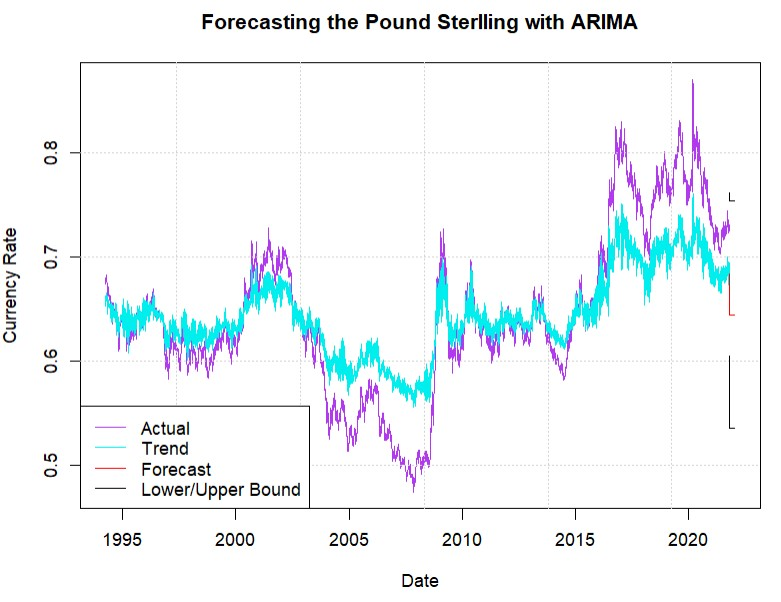
\includegraphics[width=\linewidth]{fore1.jpg} 
 \end{minipage} 
 \hspace{0.1cm} 
 \begin{minipage}[t]{8.2cm} 
 \centering 
 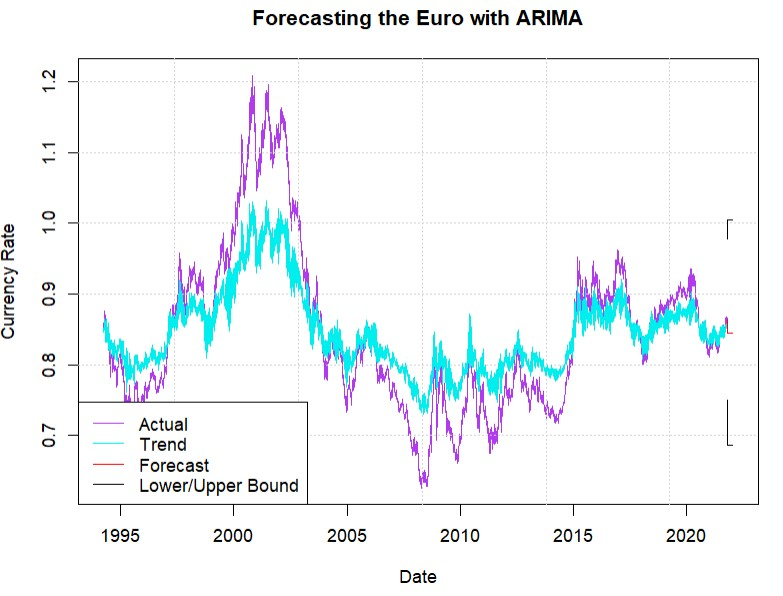
\includegraphics[width=\linewidth]{fore2.jpg} 
 \end{minipage}
\caption{Forecasting Results (1)}
\label{for1}
\end{figure}

\begin{figure}
\centering
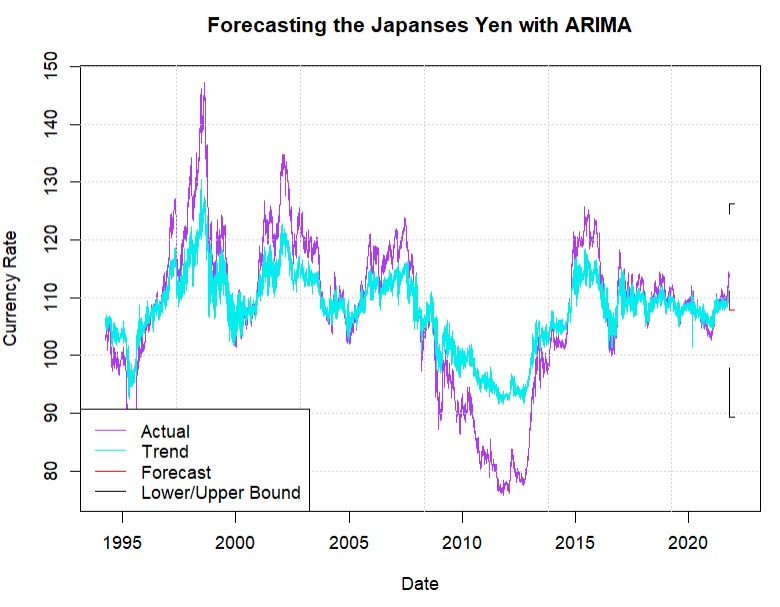
\includegraphics[scale=0.5]{fore3.jpg}
\caption{Forecasing Results (2)}
\label{for2}
\end{figure}

\newpage

\hypertarget{conclusion}{%
\section{Conclusion}\label{conclusion}}

This paper uses 33 emerging and domestic market currency rates to
determine which macroeconomic variables are most important when
analysing currency rates. Since economic models are accompanied with
many short comings, such as being overly restrictive, this paper uses a
principal component analysis technique to reduce the dimensionality of
the datasets in an interpretable way while minimizing information loss.
The paper concludes that shocks to commodity prices, such as an oil
price shock, political instability and the growth of Asian markets
should all be used to build prediction models of sport returns.

\newpage

\hypertarget{references}{%
\section*{References}\label{references}}
\addcontentsline{toc}{section}{References}

\hypertarget{refs}{}
\begin{CSLReferences}{1}{0}
\leavevmode\vadjust pre{\hypertarget{ref-akin}{}}%
Akincilar, A., TEMIZ, I. \& Sahin, E. 2011. An application of exchange
rate forecasting in turkey. \emph{Gazi University Journal of Science}.
24(4):817--828.

\leavevmode\vadjust pre{\hypertarget{ref-beck2020}{}}%
Beckmann, J., Czudaj, R.L. \& Arora, V. 2020. The relationship between
oil prices and exchange rates: Revisiting theory and evidence.
\emph{Energy Economics}. 88:104772.

\leavevmode\vadjust pre{\hypertarget{ref-can2021}{}}%
Candila, V., Maximov, D., Mikhaylov, A., Moiseev, N., Senjyu, T. \&
Tryndina, N. 2021. On the relationship between oil and exchange rates of
oil-exporting and oil-importing countries: From the great recession
period to the COVID-19 era. \emph{Energies}. 14(23):8046.

\leavevmode\vadjust pre{\hypertarget{ref-castro}{}}%
Castro, C. \& Jimenez-Rodriguez, R. 2020. Dynamic interactions between
oil price and exchange rate. \emph{PloS one}. 15(8):e0237172.

\leavevmode\vadjust pre{\hypertarget{ref-higg}{}}%
Higgins, M.L., Hysenbegasi, A. \& Pozo, S. 2004. Exchange-rate
uncertainty and workers' remittances. \emph{Applied Financial
Economics}. 14(6):403--411.

\leavevmode\vadjust pre{\hypertarget{ref-jolli}{}}%
Jolliffe, I.T. \& Cadima, J. 2016. Principal component analysis: A
review and recent developments. \emph{Philosophical Transactions of the
Royal Society A: Mathematical, Physical and Engineering Sciences}.
374(2065):20150202.

\leavevmode\vadjust pre{\hypertarget{ref-levis}{}}%
Levis, M. 1979. Does political instability in developing countries
affect foreign investment flow? An empirical examination.
\emph{Management International Review}. 59--68.

\leavevmode\vadjust pre{\hypertarget{ref-li2015}{}}%
Li, S. \& Ma, D. 2015. Oil price and exchange rate of china--a nonlinear
granger approach. In Atlantis Press \emph{2015 international conference
on education technology, management and humanities science (ETMHS
2015)}. 95--99.

\leavevmode\vadjust pre{\hypertarget{ref-mcc2009}{}}%
McCauley, R.N. \& McGuire, P. 2009. Dollar appreciation in 2008: Safe
haven, carry trades, dollar shortage and overhedging. \emph{BIS
Quarterly Review December}.

\leavevmode\vadjust pre{\hypertarget{ref-pojar}{}}%
Pojarliev, M. \& Levich, R.M. 2013. A new look at currency investing.
\emph{CFA Institute Research Foundation Monograph}.

\leavevmode\vadjust pre{\hypertarget{ref-pono}{}}%
Ponomareva, N., Sheen, J. \& Wang, B.Z. 2019. The common component of
bilateral US exchange rates: To what is it related? \emph{Empirical
Economics}. 56(4):1251--1268.

\leavevmode\vadjust pre{\hypertarget{ref-shen}{}}%
Shen, M.-L., Lee, C.-F., Liu, H.-H., Chang, P.-Y. \& Yang, C.-H. 2021.
An effective hybrid approach for forecasting currency exchange rates.
\emph{Sustainability}. 13(5):2761.

\leavevmode\vadjust pre{\hypertarget{ref-tana}{}}%
Tanamarttayarat, K. 2018. The world's largest financial market: forex.
\emph{Available at SSRN 3109245}.

\end{CSLReferences}

\hypertarget{appendix-a}{%
\section*{Appendix A}\label{appendix-a}}
\addcontentsline{toc}{section}{Appendix A}

\begin{table}
\begin{center}
\begin{tabular}{|c|c|c|c|} 
 \hline
 \multicolumn{2}{|c|}{Emerging Market} & \multicolumn{2}{|c|} {Developed Market} \\
 \hline
 Currency & ISO Code & Currency & ISO Code \\
 \hline
  Sol & PEN & Japanese Yen & JPY \\
 Saudi riyal & SAR &  Hong Kong dollar & HKD \\
 New Taiwan dollar & TWD & Canadian dollar & CAD \\
 Czech koruna & CZK & Danish krone & DKK \\
 South Korean won & KRW & Euro & EUR \\
 Renminbi & CNY & Australian dollar & AUD \\
 Indian rupee & INR &  New Zealand dollar & NZD \\
 Brazilian real & BRL & Singapore dollar & SGD \\
 Turkish lira & TRY &  Swedish Krona & SEK  \\
 Russian ruble & RUB & Norwegian krone & NOK \\
 South African rand & ZAR & Isreali Shekel & ILS \\
 Mexican peso & MXN & Pound sterling & GBP \\
 Columbian peso & COP & & \\
 Egyptian pound & EGP & & \\
 Chilean peso & CLP & & \\
 Hungarian forint & HUF & & \\
 Malaysian ringgit & MYR & & \\
 Phillipine peso & PHP & & \\
Thai bath & THB & & \\
United Arab Emirates dirham & AED & & \\
Polish złoty & PLN & & \\
\hline
\end{tabular}
\caption{Description of currencies}
 \label{cncy}
\end{center}
\end{table}

\begin{figure}
\centering
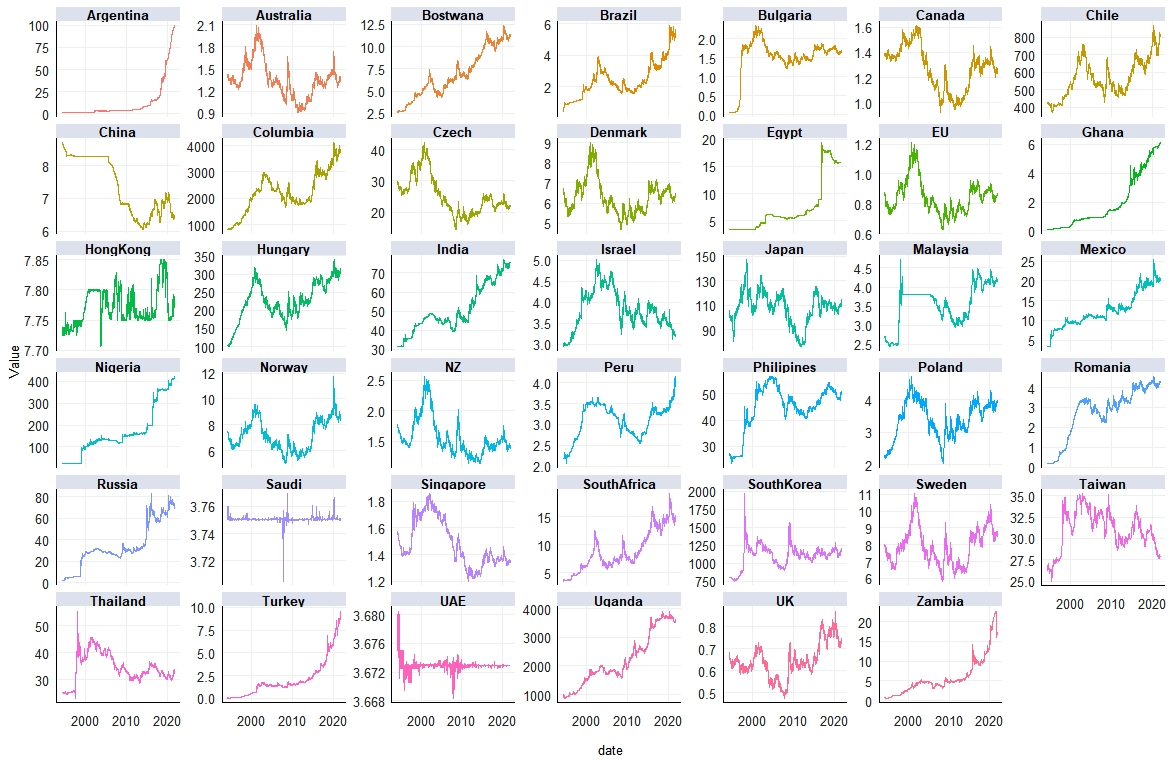
\includegraphics[scale=0.55]{descriptive.jpg}
\caption{Currency rates of all 33 emerging and developing market countries}
\label{data}
\end{figure}

\hypertarget{apprendix-b}{%
\section*{Apprendix B}\label{apprendix-b}}
\addcontentsline{toc}{section}{Apprendix B}

\begin{table}
\begin{center}
\begin{tabular}{|c|c|c|} 
 \hline
 & Correlation & P-value  \\
 \hline
 HUF & 0.9262878 & 0.000000e+00 \\
 MYR & 0.9114497 & 0.000000e+00 \\
 CLP & 0.9065261 & 0.000000e+00 \\
 PEN & 0.8988561 & 0.000000e+00 \\
 PLN & 0.8780890 & 0.000000e+00 \\
 COP & 0.8751020 & 0.000000e+00 \\
 NOK & 0.8378328 & 0.000000e+00 \\
 SEK & 0.8330755 & 0.000000e+00 \\
 BRL & 0.8263736 & 0.000000e+00 \\
 RUB & 0.7871421 & 0.000000e+00 \\
 ZAR & 0.7857282 & 0.000000e+00 \\
 INR & 0.7411845 & 0.000000e+00 \\
 PHP & 0.7307233 & 0.000000e+00 \\
 MXN & 0.6843628 & 0.000000e+00 \\ 
 TRY & 0.6753067 & 0.000000e+00 \\
 EUR & 0.6577914 & 0.000000e+00 \\
 DKK & 0.6479256 & 0.000000e+00 \\
 KRW & 0.6422958 & 0.000000e+00 \\
 GBP & 0.6259090 & 0.000000e+00 \\
 EGP & 0.6216001 & 0.000000e+00 \\
 AUD & 0.5593268 & 0.000000e+00 \\
 THB & 0.5319724 & 0.000000e+00 \\
 HKD & 0.5177139 & 0.000000e+00 \\
 TWD & 0.4758927 & 0.000000e+00 \\
 CAD & 0.4283742 & 3.557371e-319 \\
 JPY & 0.4241386 & 2.822415e-319 \\
 NZD & 0.3989511 & 3.069525e-273 \\
 ILS & 0.3742421 & 4.183071e-238 \\
 SGD & 0.2588114 & 1.665786e-110 \\
 CZK & 0.2551624 & 2.320584e-107 \\
 AED & 0.2038677 & 2.137731e-68 \\
 SAR & 0.1573449 & 3.994842e-41 \\
 CNY & -0.1710389 & 2.206939e-48 \\
\hline
\end{tabular}
\caption{Correlation and P-value for the first principal component }
 \label{pca1}
\end{center}
\end{table}

\begin{table}
\begin{center}
\begin{tabular}{|c|c|c|} 
 \hline
 & Correlation & P-value  \\
 \hline
SGD & 0.90321526 & 0.000000e+00 \\
CZK & 0.87653914 & 0.000000e+00 \\
CNY & 0.86382354 & 0.000000e+00 \\
NZD & 0.83337067 & 0.000000e+00 \\
AUD & 0.75831445 & 0.000000e+00 \\
CAD &  0.71356174 & 0.000000e+00 \\
DKK & 0.63254705 & 0.000000e+00 \\
EUR & 0.62951387 & 0.000000e+00 \\
THB &  0.59809540 & 0.000000e+00 \\
JPY  & 0.53230115 & 0.000000e+00 \\
ILS & 0.48051271 & 0.000000e+00 \\
TWD & 0.42403389 & 4.168569e-312 \\
SEK & 0.35444999 & 4.308577e-212 \\
PLN & 0.26203282 & 2.533385e-113 \\
NOK & 0.19878697 & 4.705671e-65 \\
KRW & 0.14350307 & 1.991097e-34 \\
PEN & 0.11407789 & 2.773568e-22 \\
AED & -0.03178834 & 6.993189e-03 \\
MYR & -0.03679994 & 1.792246e-03 \\
HKD & -0.04911994 & 3.056982e-05 \\
PHP & -0.11881763 & 4.754379e-24 \\
HUF &  -0.13573551 & 6.020449e-31 \\
CLP & -0.21440682 & 1.272391e-75 \\
GBP &  -0.27266672 & 6.567991e-123 \\
COP & -0.36995837 & 2.561588e-232 \\
BRL & -0.43981305 & 0.000000e+00 \\
ZAR & -0.55307034 & 0.000000e+00 \\
RUB & -0.58376817 & 0.000000e+00 \\
INR & -0.62851292 & 0.000000e+00 \\
TRY & -0.64001397 & 0.000000e+00 \\
EGP & -0.64775485 & 0.000000e+00 \\
MXN & -0.69994979 & 0.000000e+00 \\
\hline
\end{tabular}
\caption{Correlation and P-value for the second principal component }
 \label{pca2}
\end{center}
\end{table}

\begin{table}
\begin{center}
\begin{tabular}{|c|c|c|} 
 \hline
 & Correlation & P-value  \\
 \hline
ILS & 0.69659804 & 0.000000e+00 \\
TWD & 0.68427216 & 0.000000e+00 \\
PHP & 0.61977923 & 0.000000e+00 \\
THB & 0.53049506 & 0.000000e+00 \\
HKD & 0.30858474 & 1.310000e-158 \\
KRW & 0.28839441 & 6.692788e-138 \\
PEN &  0.28634486 & 6.840019e-136 \\
SGD & 0.22758825 & 3.214148e-85 \\
MYR & 0.22365740 & 2.722457e-82 \\
COP & 0.17404390 & 4.636722e-50 \\
AED & 0.09417778 & 1.179695e-15 \\
CLP & 0.08433068 & 7.709335e-13 \\
RUB & -0.02629516 & 2.568733e-02 \\
PLN & -0.04475238 & 1.458206e-04 \\
HUF & -0.07070644 & 1.909999e-09 \\
CNY &  -0.08335190 & 1.413117e-12 \\
INF &  -0.09077720 & 1.198224e-14 \\
ZAR & -0.10617861 & 1.681325e-19 \\
NZD & -0.14852069 & 8.807498e-37 \\
TRY & -0.15874418 & 7.742415e-42 \\
EGP & -0.18399169 & 7.806200e-56 \\
AUD & -0.20033914 & 4.582160e-66 \\
SAR & -0.25871186 & 2.032612e-110 \\
EUR & -0.29838703 & 6.100743e-148 \\
DKK &  -0.31163124 & 7.020576e-162 \\
SEK & -0.32101610 & 3.342782e-172 \\
CZK &  -0.34533690 & 1.002528e-200 \\
CAD & -0.44548362 & 0.000000e+00 \\
NOK &  -0.47271370 & 0.000000e+00 \\
GBP &  -0.61500908 & 0.000000e+00 \\
\hline 
\end{tabular}
\caption{Correlation and P-value for the third principal component}
 \label{pca3}
\end{center}
\end{table}

\bibliography{Tex/ref}





\end{document}
